\begin{frame}[allowframebreaks]{\underline{Methodology} -}
    \section{Methodology}
Equation \ref{2D_airfoil_thickness} represents the formula to obtain the half-thickness of symmetric NACA four-digits airfoil.
\begin{equation}
y_{t}=5 t\left[0.2969 \sqrt{x}-0.1260 x-0.3516 x^{2}+0.2843 x^{3}-0.1015 x^{4}\right]
\label{2D_airfoil_thickness}
\end{equation}
\parbox{0.55\linewidth}{
where,\\
\begin{itemize}
\item $x$ is position along the chord from 0 to 1.\\
\item $y_t$ is the half thickness for a given $x$.\\
\item $t$ is the maximum thickness represented in terms of chord.
\end{itemize}

\begin{itemize}
\item Modifying the last coefficient to -0.1036 will result in sharp trailing edge.
\item Let ($x_U$, $y_U$), and ($x_L$, $y_L$) presents the upper and the lower airfoil surface coordinates respectively. Since the airfoil is symmetric, $y_c$ is equal zero.
\end{itemize}

This results in the airfoil coordinates as shown in equation \ref{2d_final_points}.
\begin{equation}
\begin{array}{ll}
x_{U}=x & y_{U}= +y_{t} \\
x_{L}=x & y_{L}= -y_{t}
\end{array}
\label{2d_final_points}
\end{equation}
The cosine function for rectifying leading edge points:
\begin{equation}
    \begin{array}{l}
        x = 1 - \cos{\theta}  \\
        \forall  \theta \in \left(0, \frac{\pi}{2}\right)
    \end{array}
\label{cosine_function}
\end{equation}

}
\parbox{0.4\linewidth}{
\begin{figure}  
    \centering
    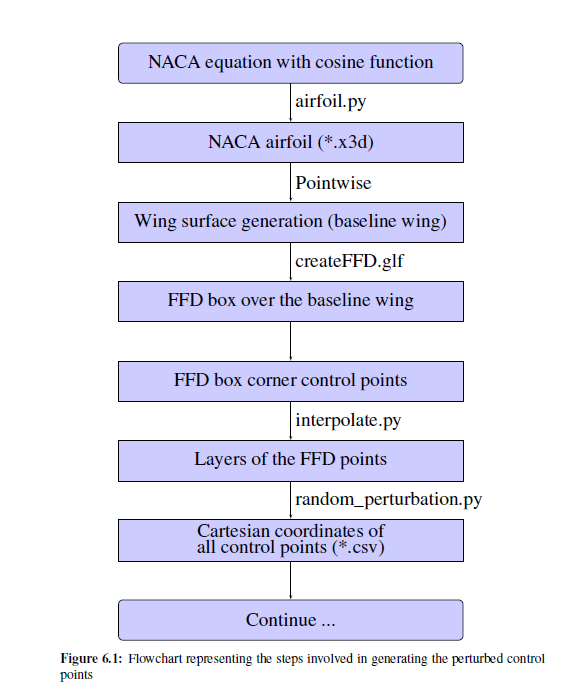
\includegraphics[scale = 0.25]{figures/flow_chart_1.png}
\end{figure}
}
\parbox{0.45\linewidth}{
\begin{figure}  

    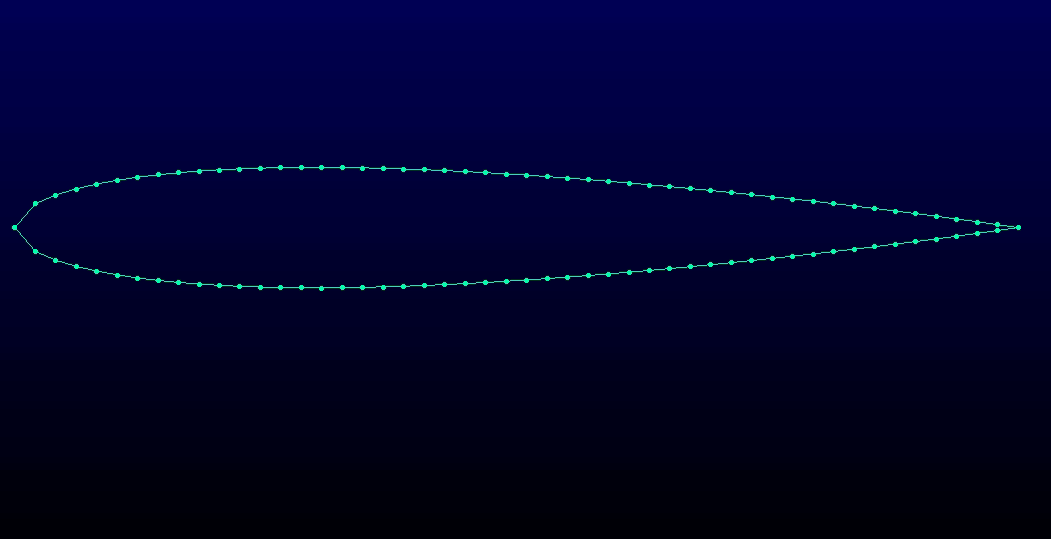
\includegraphics[scale = 0.12]{figures/airfoil_uniform_points.png}
    \caption{Uniform distribution of points along horizontal direction [total 100 grid points].}
    \label{uniform_points_airfoil}
\end{figure}
}
\parbox{0.45\linewidth}{
\begin{figure}  
    \centering
    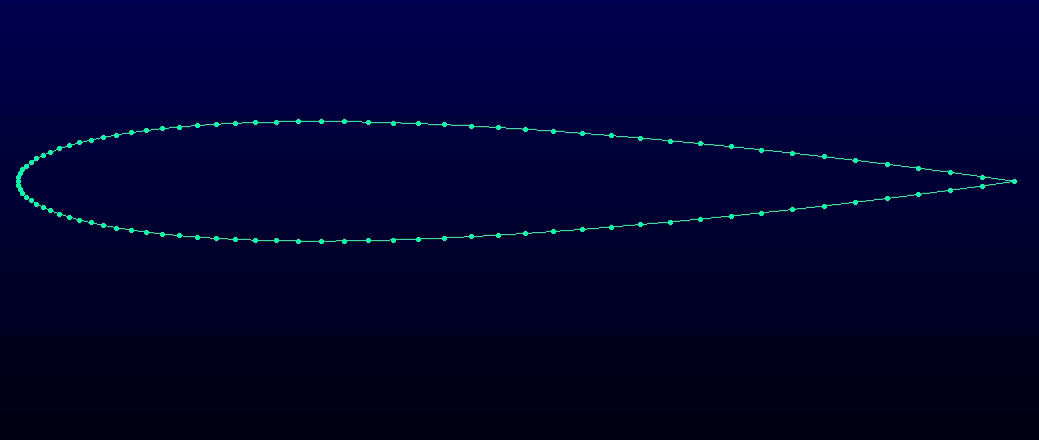
\includegraphics[scale = 0.13]{figures/airfoil_cosine.png}
    \caption{Cosine function distribution of points along horizontal direction [total 100 grid points].}
    \label{cosine_points_airfoil}
\end{figure}
}
\parbox{0.4\linewidth}{
\begin{itemize}
\item Import the cosine distribution airfoil into Pointwise.
\item Extrude in third dimension (span direction) results in baseline wing.
\item 200 mesh points are chosen along the span direction.
\item Export back in Plot3D format.
\end{itemize}
}
\parbox{0.5\linewidth}{
\begin{figure}
    \centering
    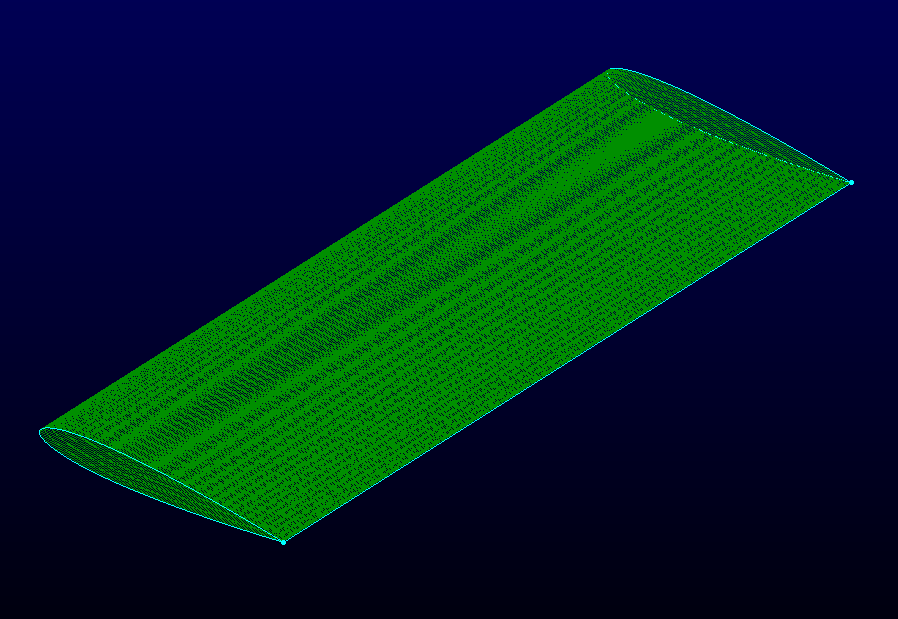
\includegraphics[scale=0.15]{figures/wing_3d.png}
    \caption{NACA0012 surface mesh (300 $\times$ 200) grid points.}
    \label{naca0012 wing mesh}
\end{figure}
}
\parbox{0.45\linewidth}{
\begin{figure}
    \centering
    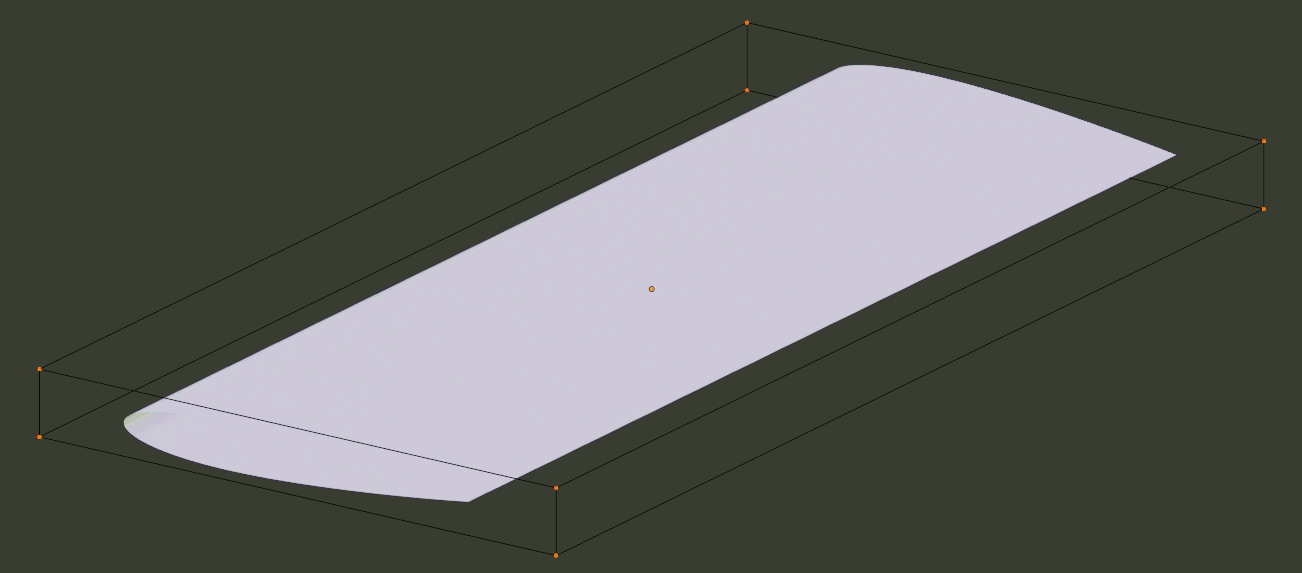
\includegraphics[scale=0.1]{figures/wing_FFD_corner_pt.png}
    \caption{FFD box coupled with NACA0012 wing surface. Corner points highlighted act as control points.}
    \label{ffd_wing_corner}
\end{figure}
}
\parbox{0.47\linewidth}{
\begin{figure}
    \centering
    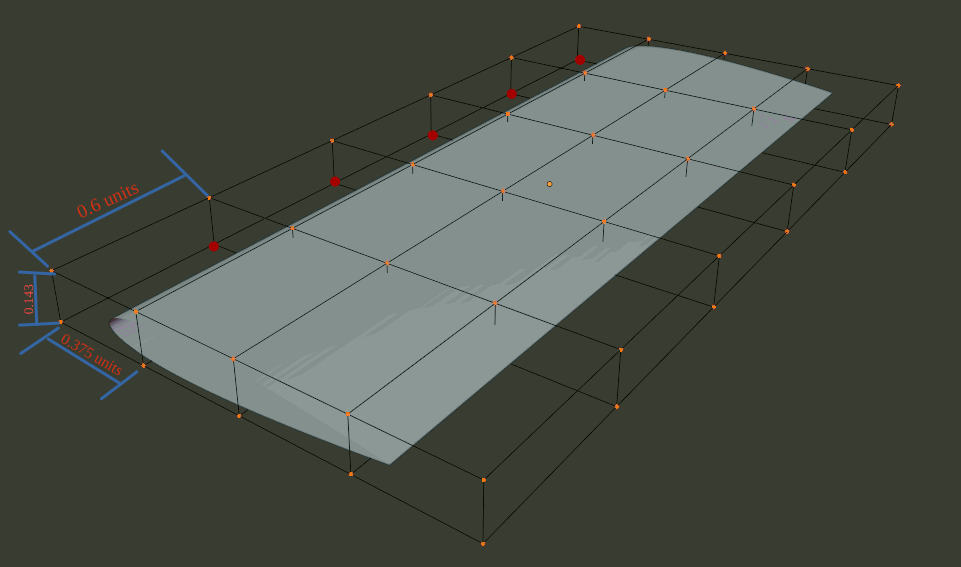
\includegraphics[scale=0.13]{figures/wing_all_cp_FFD.png}
    \caption{FFD box along with interpolated points and corner points.}
    \label{ffd_wing_interpolate}
\end{figure}
}
\begin{itemize}
\item Glyph script is used to generate and extract the FFD corner points coordinates.
\item Scale factor of 1.5 is used along the chord direction. 
\item Along thickness and span direction,  a scale factor of 1.1 and 1 unit is used.
\item However, with just corner control points, it is not possible to obtain more featured wings.
\item Additional control points are induced as layers.
\item A total of 5 equidistant control points along chord, 2 along thickness, and 6 along span direction is added, resulting total of 60 control points. 
\item Each control point can be perturbed in three direction (x, y, z directions)
\item This results in the 180 dimension problem (60*3).
\end{itemize}
\underline{Control points perturbation:}
\begin{equation}
\begin{array}{lll}
s_i = \frac{x_i - x_{origin}}{\Delta x}, & t_i = \frac{y_i - y_{origin}}{\Delta y}, & u_i = \frac{z_i - z_{origin}}{\Delta z} 
\end{array}
\label{parameter_equation}
\end{equation}

where,\\
\begin{itemize}
\item $s_i$, $t_i$, $u_i$ are the parametric form of $i^{th}$ mesh point. \\
\item $x_i$, $y_i$, $z_i$ are the cartesian form of $i^{th}$ mesh point. \\
\item $x_{origin}$, $y_{origin}$, $z_{origin}$ are the cartesian coordinates of the selected FFD box corner point. \\
\item $\Delta x$, $\Delta y$, $\Delta z$ are the differences between extreme points coordinates in the FFD box.\\[1mm]
\end{itemize}
Wing surface is mapped from cartesian system to parametric system.\\[1mm]

Allowing all control points to perturb would result in infeasible wings. Few of control points need to be limited.


\begin{itemize}
\item The control points at the wing root section are restricted in the chord and thickness direction only $\implies$ dimension reduction by 10.
\item The control points from layer 1 to layer 5 can perturb by the same values in the span direction $\implies$dimension reduction by 45.
\item Overall the problem dimension becomes 125 (180 - 55).
\end{itemize}
 
 Allowed control points are perturbed by a value.
\begin{itemize}
\item  $\leq$ 0.1875 unit along chord direction.
\item  $\leq$ 0.07 unit along thickness direction.
\item  $\leq$ 0.3 unit along span direction.
\end{itemize}
\newpage
Figure  \ref{ffd_box_perturbed} illustrate one of the wing obtained.
\parbox{0.47\linewidth}{
\begin{figure}
    \centering
    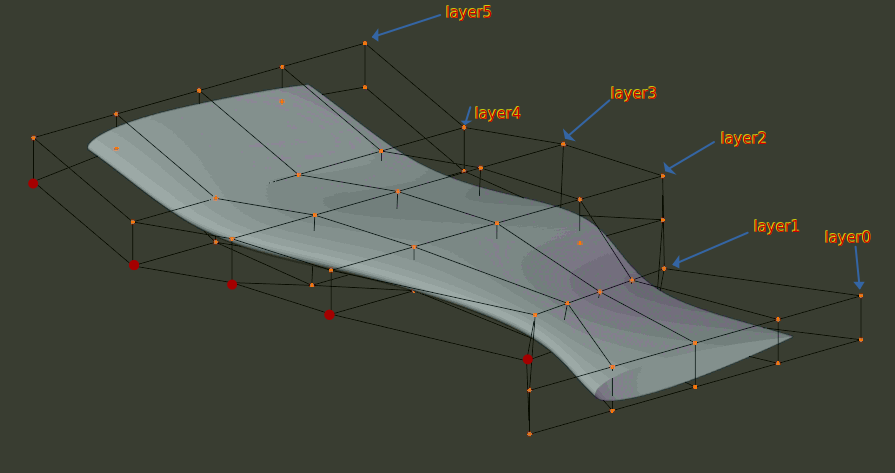
\includegraphics[scale=0.15]{figures/wing_FFD-_displaced.png}
    \caption{Effect of control points perturbation on the wing surface.}
    \label{ffd_box_perturbed}
\end{figure}
}
\parbox{0.47\linewidth}{
\begin{figure}
    \centering
    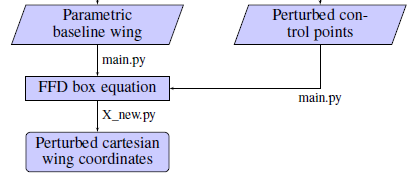
\includegraphics[scale=0.3]{figures/ffd_box_equation.png}
    \caption{Block diagram representing the input and output to FFD box equation.}
\end{figure}
}
\begin{itemize}
\item A 1000 set of perturbed control points are randomly generated and result in 1000 perturbed wings. 
\item Each wing is represented by 30000 surface mesh points $\implies$ a matrix of 1000 $\times$ 90000 is created.
\item These perturbed wings are subjected PCA analysis.
\item Outcome of PCA result in three matrices. 
\item Analyzing the diagonal matrix and calculating the scatter energy resulted in dimension reduction of 20 as shown in table \ref{scatter_energy}.
\end{itemize}


$$E=\sum_{i=1}^{m p} \lambda_{i}^{2}$$

where,\\
\begin{itemize}
\item $\lambda_i$ is the $i^{th}$ diagonal entry of $\Sigma$. 
\item Selecting the first few modes from the matrix $M$ and taking note of their corresponding eigenvalues makes it possible to predict the amount of scatter energy being captured.
\end{itemize}

\parbox{0.43\linewidth}{
\begin{figure}   
    \centering
    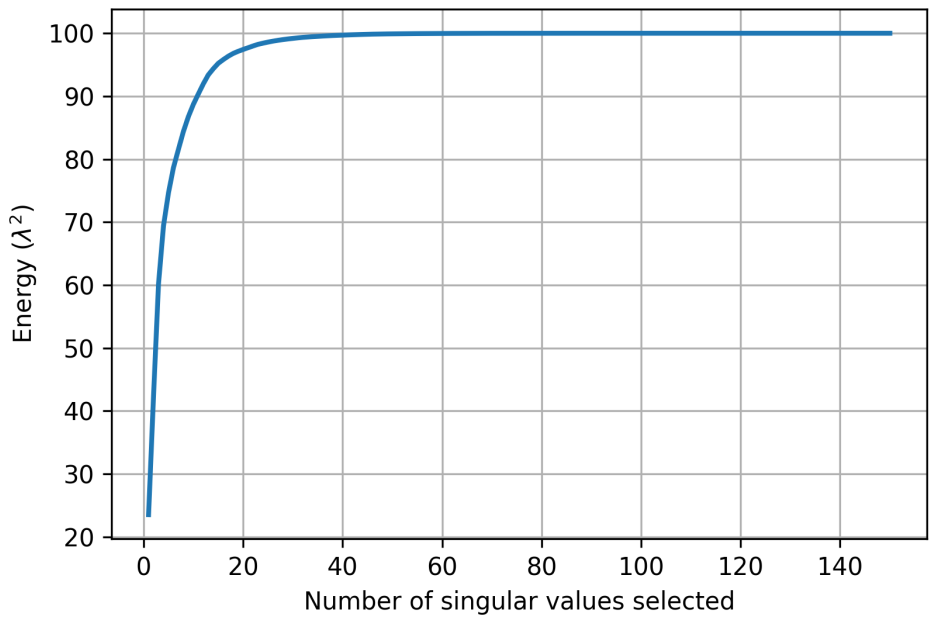
\includegraphics[scale=0.13]{figures/energy_plot.png}
    \caption{Scatter energy verses number of singular values selected.}
    \label{energy plot}
\end{figure}
}
\parbox{0.46\linewidth}{
\begin{table}
    \centering
    \begin{tabular}{|c|c|}
        \hline
        Singular values selected & Scatter energy ($\%$) \\\hline
         1 & 23.52\\
         2 & 42.48\\
         5 & 74.63\\
         10 & 88.70\\
         \textbf{20} & \textbf{97.42}\\
         30 & 99.17\\
         50 & 99.98\\ \hline
    \end{tabular}
    \caption{Singular value selected against scatter energy}
    \label{scatter_energy}
\end{table}
}
\newpage
For example, let $t$ be the number of leading principal components being selected. The matrix $X^*$ will be a matrix multiplication between $U_s$, $\Sigma_s$, and $V^T_s$. that is, $$X^* = U_s \Sigma_s V^T_s$$

where,\\
$U_s$ is the matrix consisting of first $t$ columns (1000 $\times$ $t$).\\
$\Sigma_s$ is the diagonal vector with $t$ elements ($t$ $\times$ $t$).\\
$V^T_s$ is the matrix with first $t$ rows ($t$ $\times$ 90000).\\[1mm]

\underline{Generating initial population:}
\begin{itemize}
    \item Finding maximum and minimum of first 20 columns of matrix $U_s$.
    \item This space act as design space for the optimization.
    \item Generate 20 set of random number between the given design space $U_s$.
    \item Find $X^*$ as shown above, and append it to baseline wing and average error vector.
    \item This result in 20 initial population.
\end{itemize}
$$ M = x^0 + \bar{x} + X^* $$
$M$ is as called a reduced-order model.
\newpage
\parbox{0.43\linewidth}{
\begin{figure}
    \centering
    \framebox{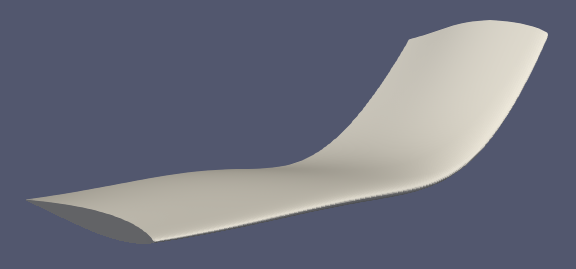
\includegraphics[scale=0.2]{figures/svdwing1.png}}
    \caption{General SVD wing 1.}
    \label{svd_wing_1}
\end{figure}
}
\parbox{0.43\linewidth}{
\begin{figure}
    \centering
    \framebox{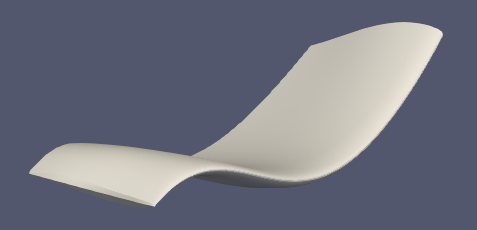
\includegraphics[scale=0.25]{figures/svdwing_2.png}}
    \caption{General SVD wing 2.}
    \label{svd_wing_2}
\end{figure}
}
\underline{Using Glyph script:}
\begin{itemize}
\item Glyph script import perturbed wing.
\item Based on the span size, the winglet is generated and appended into the perturbed wing.
\item The volume mesh is generated with 15 chord units in all directions.
\end{itemize}

\parbox{0.47\linewidth}{
\begin{figure}
    \centering
    \framebox{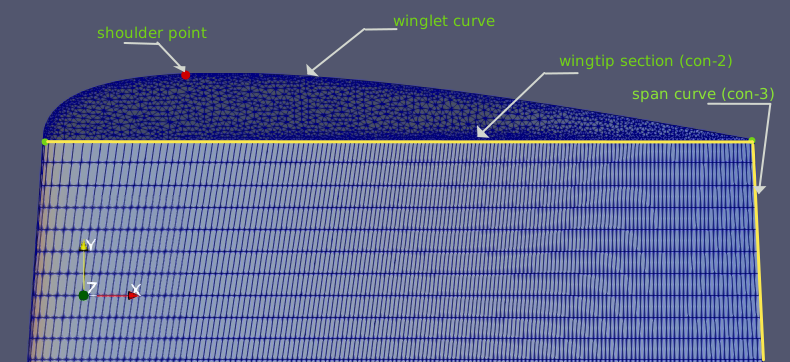
\includegraphics[scale = 0.15]{figures/winglet_frontview.png}}
    \caption{Winglet frontview.}
    \label{winglet_frontview}
\end{figure}
}
\parbox{0.47\linewidth}{
\begin{figure}
    \centering
    \framebox{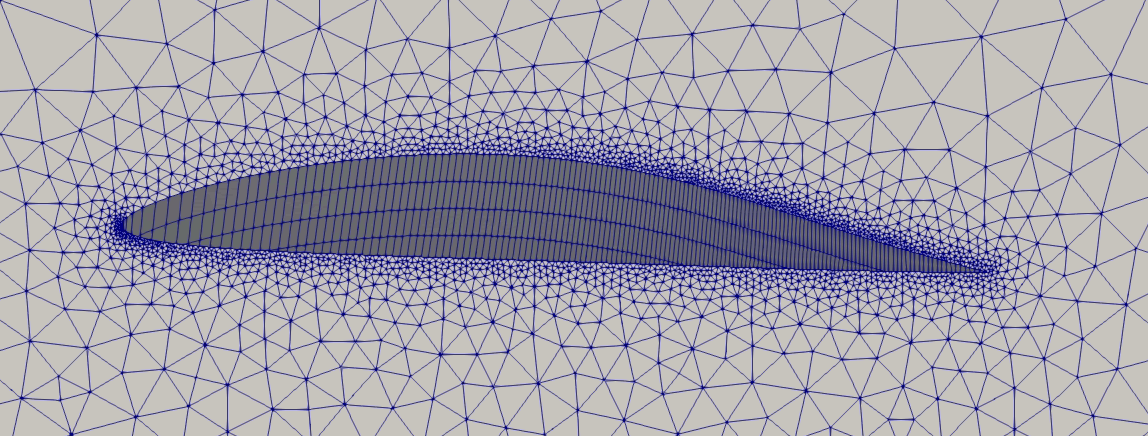
\includegraphics[scale = 0.12]{figures/airfoil_mesh.png}}
    \caption{Mesh around one of perturbed wing sectioned at symmetry plane.}
    \label{airfoil_mesh}
\end{figure}
}
\begin{itemize}
\item The wing surface (including winglet) is marked as Euler wall.
\item Wall surface at root section is marked as Symmetry wall. 
\item Rest of all boundary surfaces are marked as far field.
\end{itemize}

\parbox{0.4\linewidth}{
\begin{figure}
    \centering
    \framebox{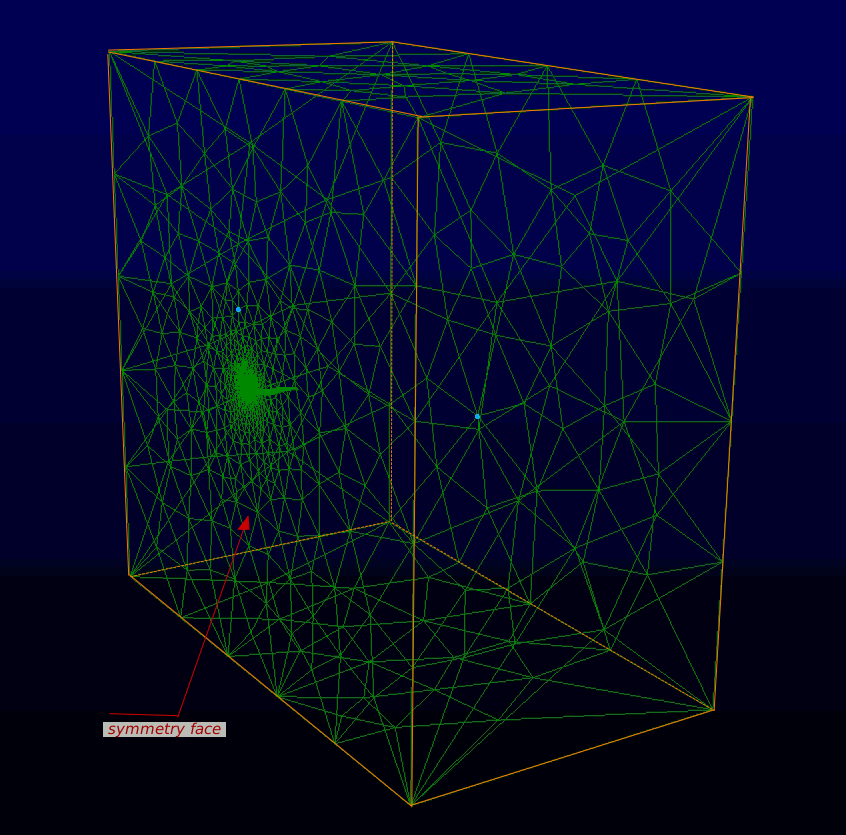
\includegraphics[scale = 0.15]{figures/volume_mesh.png}}
    \caption{T-Rex mesh}
    \label{T-Rex}
\end{figure}
}
\parbox{0.57\linewidth}{
\begin{figure}
    \centering
    \framebox{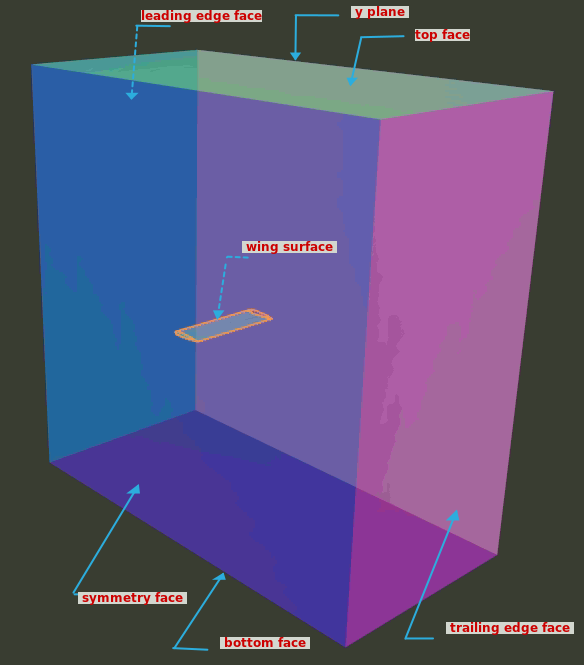
\includegraphics[scale = 0.19]{figures/wing_body.png}}
    \caption{Far field boundaries.}
    \label{farfield}
\end{figure}
}
\begin{itemize}
\item After generation volume mesh, the 20 population is subjected to optimization with fNRAND1 algorithm.  
\end{itemize}
\end{frame}